
% book example for classicthesis.sty
\documentclass[
  % Replace twoside with oneside if you are printing your thesis on a single side
  % of the paper, or for viewing on screen.
  oneside,
  %twoside,
  11pt, a4paper,
  footinclude=true,
  headinclude=true,
  cleardoublepage=empty
]{scrbook}

\usepackage{lipsum}
\usepackage[linedheaders,parts,pdfspacing]{classicthesis}
\usepackage{amsmath}
\usepackage{amsthm}
\usepackage{mathtools}
\usepackage{acronym}
\usepackage{dissertation}
\usepackage{multirow}
\usepackage{pdfpages}
%\usepackage[acronym]{glossaries}

% Title
\title{Advanced Light Transport Algorithms on Heterogeneous Platforms: evaluation of the DICE framework}

% Author
\author{César Morais Perdigão}

% Supervisor
\def\supervisor{%
	Luís Paulo Peixoto dos Santos
\\
	Alberto José G. de C. Proença
}

% Date
\date{\today}

%%Defines
%\def \... {..}

\makeglossaries  %  either use this ...

%\makeindex	% ... or this

\newcommand*{\myglossaryindent}{0.65cm}         
\newcommand*{\myglsdescwidth}{10cm}                     
\newglossarystyle{altlong4colwithindent}
{
  \glossarystyle{altlong4col}
  \renewenvironment{theglossary}
    {\begin{tabular}[l]{@{\hspace{\myglossaryindent}}lp{\myglsdescwidth}lp{\glspagelistwidth}@{}}}
    {\end{tabular}}
}

\begin{document}
	
% Add acronym definitions
\newacronym{vcm}{VCM}{Vertex Connection and Merging}
\newacronym{mlt}{MLT}{Metropolis Light Transport}
\newacronym{pt}{PT}{Path Tracing}
\newacronym{bdpt}{BDPT}{Bidirectional Path Tracing}
\newacronym{pm}{PM}{Photon Mapping}
\newacronym{ppm}{PPM}{Progressive Photon Mapping}
\newacronym{bpm}{BPM}{Bidirectional Photon Mapping}

\newacronym{mis}{MIS}{Multiple Importance Sampling}

\newacronym{cpu}{CPU}{Central Processing Unit}
\newacronym{gpu}{GPU}{Graphics Processing Unit}

\newacronym{mcmc}{MCMC}{Markov Chain Monte Carlo}

\newacronym{mic}{MIC}{Many Integrated Core}

\newacronym{sse}{SSE}{Streaming SIMD Extensions}
\newacronym{avx}{AVX}{Advanced Vextor Extensions}
\newacronym{simd}{SIMD}{Single Instruction Multiple Data}
    
% Cover page ---------------------------------------------
\sf
	\pagenumbering{alph}
	\thispagestyle{empty}
	%!TEX root = dissertation.tex

\makeatletter

% UM_ENg Logo
\def\UMEng#1#2{\begin{tikzpicture}[
	% bars styling,
	logone/.style={rectangle,fill=white,rounded corners=0.08cm,minimum width=0.16cm,inner sep=0pt},
	bigone/.style={minimum height=0.74cm},
	smaone/.style={minimum height=0.48cm},
	engone/.style={minimum height=0.86cm},
	pos1/.style={xshift=1.3cm,yshift=1.3cm},
	pos2/.style={xshift=3.9cm,yshift=1.3cm}]
	
% Uminho logo
	\fill[fill=#1] (0,0) -- (2.6,0) -- (2.6,2.6) -- (0,2.6) -- cycle;
	\foreach \i in {1,...,3}{
		\node at (\i*120+30:0.45)[logone,bigone,pos1,rotate=\i*120-60]{};
		\node at (\i*120+90:0.60)[logone,smaone,pos1,rotate=\i*120]{};
	}

% EngUminho logo
	\fill[fill=#2] (2.6,0) -- (5.2,0) -- (5.2,2.6) -- (2.6,2.6) -- cycle;
	\foreach \i in {1,...,5}
		\node at (\i*72-90:0.74)[engone,logone,pos2,rotate=\i*72-90]{};
\end{tikzpicture}}

\def\yyy#1{\fontfamily{phv}\fontseries{mc}\selectfont {\ifnum\hide=1\relax\else#1\fi}}
\def\xxx#1{\fontfamily{phv}\fontseries{mc}\selectfont #1}
\def\zzz#1{\fontfamily{phv}\fontseries{mc}\fontseries{b}\selectfont #1}
\def\kkk#1{\fontfamily{phv}\fontseries{mc}\fontseries{b}\selectfont {\ifnum\hide=1\relax\else#1\fi}}

\long\def\coverEtc{
%Logo
~\vskip-2cm\rule{4cm}{0pt}\begin{tabular}{l}
\UMEng\umc{eng}
\\\zzz{Universidade do Minho}\rule{0pt}{1cm}
\\\xxx{}{Escola de Engenharia}
\\\xxx{Departamento de  Informática}
\\\rule{0pt}{4cm}
\\\xxx{{\Large\@author}}
\\\rule{0pt}{1em}
\\\zzz{\Large\@titleA}
\\\zzz{\Large\@titleB}
\\\zzz{\Large\@titleC}
\\\rule{0pt}{5cm}
\\\yyy{\large Dissertação de Mestrado}
\\\yyy{\large Mestrado em Engenharia Informática}
\\\rule{0pt}{6mm}
\\\yyy{\large Trabalho realizado sob a orientação de}
\\\kkk{\@supervisor}\rule{0pt}{4mm}
\\\kkk{\@cosupervisor}
\\\rule{0pt}{2cm}
\\\xxx{{\small\@date}}
\end{tabular}
}


\begin{frontcover}
\gdef\umc{um}\gdef\hide{1}
\thispagestyle{empty} \pagecolor{grey} \textcolor{white} \coverEtc
\end{frontcover}

\begin{titlepage}
\gdef\umc{um}
\gdef\hide{0}
\thispagestyle{empty} \pagecolor{white}\textcolor{grey} \coverEtc
\end{titlepage}

\makeatother


\rm
	\cleardoublepage
%---------------------------------------------------------
% Add acknowledgements

%\chapter*{Acknowledgements}
%Write acknowledgements here

	\cleardoublepage
	
% Add abstracts (en,pt) -----------------------------------------------------------
\chapter*{Abstract}
Physically based rendering is an unsolved challenge, as there are many efficient light transport algorithms, although none is robust enough to handle every possible situation, lighting and scene configuration. The performance of such techniques can be enhanced using two different approaches: more efficient and robust algorithms and the use of more computational power. Although most modern computers have both powerful CPUs and GPUs, most current implementations of light transport algorithms only take advantage of one of these processors. Implementing new light transport algorithms such as Vertex Connection and Merging on these hybrid platforms, using both CPU and GPU, may provide more efficient results although the suitability for such algorithms for heterogeneous computing platforms has not been tested yet, and that is the main goal of this project.

	\cleardoublepage

\chapter*{Resumo}
A sintese de imagens fotorrealistas é um desafio ainda por resolver, dado que existem muitos algoritmos de transporte de luz eficientes, porem nenhum lida com todas as situações de forma robusta. O desempenho destas técnicas pode ser melhorado usando algoritmos de transporte de luz mais eficientes e robustos bem como usando mais poder computacional. Apesar da maioria dos computadores modernos ter disponível poderosos CPU's e GPU's, a maioria das implementações utiliza apenas um destes processadores. Implementar novos algoritmos de transporte de luz tal como o Vertex Connection and Merging nestas plataformas hibridas pode trazer ganhos de desempenho, porem nenhum teste para avaliar a adequabilidade destes algoritmos para sistemas heterogéneos foi efetuado, e é esse o principal objectivo deste projeto.

	\cleardoublepage
	
	\pagenumbering{roman}
	\setcounter{page}{3}
	%pagestyle{fancy}   % -------- removed
	\rm
	
	% Document
	\cleardoublepage
    \phantomsection
    \addcontentsline{toc}{chapter}{Contents}
	\tableofcontents
	
	%\cleardoublepage
	%\listoffigures
	
	\cleardoublepage
	\listoftables
	
	%\cleardoublepage
	%\lstlistoflistings
	
	% Add list of acronyms
	\printglossary[type=\acronymtype, title=List of Acronyms, nonumberlist=true, toctitle=List of Acronyms, style=altlong4colwithindent]
	\cleardoublepage
	\pagenumbering{arabic}
	\setcounter{page}{3}

%\part{Introductory material}

\chapter{Introduction}

One of the main challenges in computer graphics is physically based rendering, the synthetic creation of images that are perceptually indistinguishable from real world views based on a geometric description of the scene, materials and light sources. There are several algorithms that try to solve this problem, although none of them is yet robust enough to handle every possible situation.

One of the first solutions, \gls{pt} proposed by \cite{Kajiya}, aims to solve this problem by tracing ligh transport paths starting from the camera until a light source is hit.

One improvement upon this algorithm was \gls{bdpt}, developed independently by \cite{Lafortune} and \cite{Veach}. Although with different mathematical background, the goal is to sample more light transport paths by connecting sub-paths generated from the camera and the light source. This allows for a much more efficient rendering of effects like caustics, although
effects like reflected caustics are still too difficult for a bidirectional path tracer to handle robustly.

%In an effort to improve the efficiency and robustness of light transport algorithms, \cite{Veach} proposed the adaptation of the metropolis sampling algorithm to the light transport problem. The metropolis algorithm consists in starting from any point in the function domain, we apply mutations to this point with a carefully chosen acceptance probability, and the sampling pattern will be proportional to the value of the function. In the case of rendering, the image function is the estimated incident radiance value for each pixel and the integration domain is the set of all light transport paths.

One completely different approach developed by \cite{Jensen} was instead of trying to find paths from the light source to the camera to just trace a packets of photons throughout the scene and store them in an acceleration structure referred to as Photon Map. In a second pass, the rays would start from the camera and consult the photon map in the vicinity of the intersections and calculate the expected radiance through a density estimation. Unlike all the previously presented methods, photon mapping introduces bias, that is, it may not converge to the correct result of the rendering equation. However, it is consistent, and by diminishing the search radius on the photon map and increasing the number of traced photons, the bias reduces to zero in the limit \citep{Hachisuka}.

Most recently, an attempt to combine these two approaches was proposed by \cite{Georgiev}. In this algorithm, \gls{vcm}, photon mapping and bidirectional path tracing are combined, taking advantage of each of the algorithms strong points: the high convergence rate from bidirectional path tracing and the better handling of caustics from photon mapping. These two algorithms are combined by reducing photon mapping to a path sampling technique in the path integration space formulation and combines it with bidirectional path tracing using \gls{mis}.

In spite of the differences between the different techniques, what they all have in common is the need for computaional power, since all of these algorithms are based on ray tracing, a computationally expensive operation.

Although most computers nowadays contain both a \gls{cpu} and a \gls{gpu}, most commonly seen implementations only use one of these processors, and so waste useful computational power. Developing for these heterogeneous platforms, such that all different devices are effectively and efficiently used by the application, raises a number of challenges. In fact, besides all issues commonly associated with parallel processing (e.g., workload decomposition, communication overheads, load balancing), the heterogeneity of the different devices often implies maintaining different implementations for each architecture as well as dealing with separate memory address spaces.
Frameworks, such as StarPU \citep{augonnet2011starpu} and DICE \citep{Barbosa} have been proposed to alleviate the application programmer from the challenges risen by heterogeneous systems. 

\section{The Problem and its Challenges}

%In order to solve these issues there is the framework DICE, developed in the University of Texas at Austin. This framework allows an easy workload distribution as well as a memory management system. Mapping light transport algorithms to these heterogeneous systems may lead to performance improvements although no test to evaluate the suitability of these algorithms has been conducted yet. 

With all this, the main goals for this project are to evaluate the suitability of the above described path integration space rendering algorithms for parallel heterogeneous systems, such as those commonly found on current desktops, I.e., multicore \gls{cpu} and a \gls{gpu}. The DICE framework has been selected for this evaluation, because it has been developed in close cooperation with our research group and we are interested on identifying its strong and weak points, regarding both performance and usability.

\chapter{Background on Computational Light Transport}

Physically based rendering is the process of generating synthetic images indistinguishable from the perception of the real world. These images are generated according to a geometric model of the scene and models for every material and light source present. With this information is possible to simulate the light transport process from the light sources to the camera through the scene in order to synthesize an image. With this simulation, the radiance for each pixel of the image is determined, being radiance the radiant power incident on a given region per area and solid angle unit.

Physically based rendering is a computationally intensive process, and the use of heterogeneous systems may provide additional computation power, at the cost of a more difficult development. This issue is addressed by frameworks such as DICE \citep{Barbosa} and StarPU \citep{augonnet2011starpu} that aim to ease the development of heterogeneous applications as well as scheduling and memory management across devices.

\section{Path Tracing}

One of the first solutions to the global illumination was introduced by \cite{Kajiya} when he defined the problem of rendering as the resolution of an integral equation, also know as the rendering equation.

\begin{equation}
I(x,x')=g(x,x')\left[e(x,x')+\int_{S}^{} \rho(x,x',x'')I(x',x'')dx''\right]
\label{eq:render_eq}
\end{equation}

Where:

\begin{tabular}{r l}
$I(x,x')$ & is related to the intensity of light passing from point $x$ to $x'$ \\
$g(x,x')$ & is the geometric term \\
$e(x,x')$ & is related to the intensity of emitted light from $x$ to $x'$ \\
$\rho(x,x',x'')$ & is related to the intensity of light scattered from $x''$ to $x$ through $x'$\\
\end{tabular}
\\

This equation translates to how much light arrives at a given point from a given direction. This integral equation can not be calculated analytically, so its expected value is calculated through Monte Carlo Integration. Based on this, the goal is to trace a light transport path, with points $x_0$ .. $x_n$ in which $x_0$ is a point on a light source and $x_n$ is a point on the camera lens. 
Commonly, these paths are traced from the camera to the light source, to ensure that paths sampled fall in the image plane and to capture reflection and refraction paths. However caustic paths have a very low sampling probability, reaching zero if using point light sources. Tracing paths form the light source to the camera however sample caustics more effectively but specular paths can not be sampled.

\begin{figure}[H]
\centering
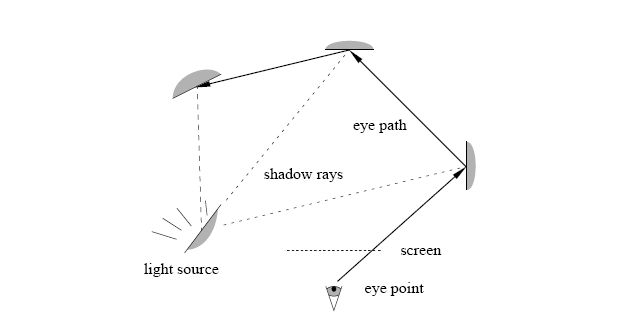
\includegraphics[width=0.75\linewidth]{img/ptDiagram.jpeg}
\caption{\label{img:ptdiag} Path Tracing Algorithm}
\end{figure}

\section{Bidirectional Path Tracing}

\gls{bdpt}, proposed independently by \cite{Veach} and \cite{Lafortune} combines both forward and backwards path tracing in one single method that can become more robust than the previous two alone. Although with a different mathematical background, both authors propose that the method should sample pairs of sub-paths containing a light sub-path and a camera sub-path. Then, each vertex of one sub-path is explicitly connected to all vertices of the other one, generating a new set of light transport paths.

\begin{figure}[H]
\centering
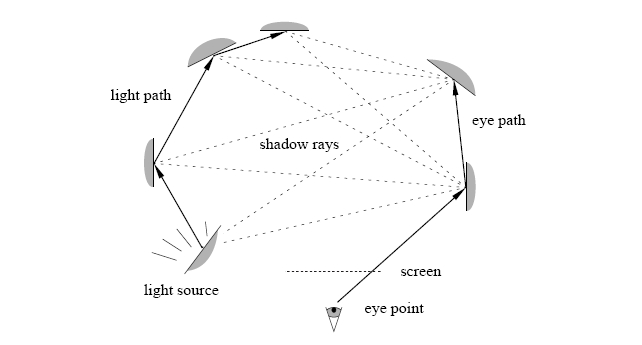
\includegraphics[width=0.75\linewidth]{img/bptDiagram.jpeg}
\caption{\label{img:bptdiag} Bidirectional Path Tracing Algorithm}
\end{figure}

In order to make the algorithm more robust, \cite{Veach} proposed the Path Space Integration Framework and \gls{mis}. The first consists in converting the problem of light transport from a recursive integral equation (~\ref{eq:render_eq}) to a simple integral over the space of all light transport paths.
\begin{equation}
I_j=\int_\Omega f_j(x)d\mu (x)
\label{eq:path_int}
\end{equation}
where $\Omega$ is the set of all light transport paths of all lengths, $\mu$ is a measure on this space of paths and $f_j$ is the measurement contribution function.

Multiple Importance Sampling is a technique that attempts to combine multiple sampling techniques in a probably good way in order to minimize variance.
\begin{equation}
F = \sum_{i=1}^n \frac{1}{n_i} \sum_{j=1}^{n_i} \omega_i (X_{i,j}) \frac{f(X_{i,j})}{p_i (X_{i,j})}
\label{eq:mis}
\end{equation}
Being $n$ the number of sampling techniques and $n_i$ the number of samples for technique $i$, this estimator attributes a weight $\omega$ to each sample. The balance heuristic is a simple and robust way to calculate these weights and is demonstrated that no other heuristic is much better \citep[p.~264]{Veach}.
\begin{equation}
\omega_i (x) = \frac{n_i p_i (x)}{\sum _k n_k p_k (x)}
\label{eq:balance}
\end{equation}
In order to use \gls{mis} in Bidirectional Path Tracing one must consider that each path of a given length can be sampled in several ways: a path of length $n$ can be sampled by using whatever light and camera sub-paths of $s$ and $t$ vertices as long as $n=s+t+1$. Given this it is just needed to apply the heuristic above to calculate the respective weight for that path.

\begin{equation}
I=\sum_{s \geq 0}\sum_{t \geq 0}\omega_{s,t}(x_{s,t})\frac{f_j (x_{s,t})}{p_{s,t}(x_{s,t})}
\label{eq:bpt}
\end{equation}

This algorithm is much more robust than path tracing, as it can sample many light transport paths efficiently and robustly. Nonetheless, this algorithm is not perfect for every situation, as it has difficulty sampling reflected caustics \citep{Georgiev}.

%\section{Metropolis Light Trasport}

%In an effort to improve the efficiency of light transport algorithms, \cite{Veach} proposed the adaptation of the Metropolis Sampling algorithm to the light trasport problem. This algorithms starts from one point in the function domain and generates a random walk such that in the limit, the sampling distribution is proportional to the function value, called the stationary distribution function. These new samples however, may not allways be accepted, and have an acceptance probability given by equation ~\ref{eq:acc_prob}.
%\begin{equation}
%a(x\xrightarrow{}y) = min \left\{ 1 , \frac{f(y)T(y\xrightarrow{}x)}{f(x)T(x\xrightarrow{}y)} \right\}
%\label{eq:acc_prob}
%\end{equation}
%where $a(x\xrightarrow{}y)$ is the acceptance probability from state $x$ to $y$ and $T$ is the the transition probability for the mutation being applied. As in the limit, the samples are distributed proportionaly to the function value, all samples have the same contribution to the final result.

%Applying this algorithm to the light transport problem, the function domain is the space of light transport paths and the function value is the contribution these paths have in the final image. The \gls{mlt} algorithm starts by generating a light transport path, using \gls{bdpt} for instance, and then aply mutations to that path using the acceptance probability defined in ~\ref{eq:acc_prob}.

%As the initial sample in the algorithm was not sampled according to the stationary distribution function, the algorithm exhibits startup bias, because only in the limit the samples converge to stationary distribution function and until then the results may be heavly influenced by the choice of the initial path. This problem is solved by sampling a set of paths, assigning each a weight $W_0 = f(X_0)/p_0 (X_0)$, and then select a subset of these paths with a probability proportional to these weights. Then, all these paths are assigned the same weight that is the average of all previously sampled weights. This solves two problems: removes start-up bias and calculates the normalization weight of the samples, scaling them to the right value.

%An important part of this algorithm are the mutations. In his work, \cite{Veach} proposed a set of mutations that aimed to solve some well known problem of light transpor algorithms, namely reflected caustics. However, \cite{Kelemen} proposed a simpler and robust form of mutation in the primary sampling space. Instead of trying to directly mutate the paths, mutations would be applied to the pseudo-random numbers used to generate them, being this perturbation smaller the higher the contribution of the sample in order to keep the acceptance probability high. One important property of the mutaions used in the Metropolis algorithm is that these must be able to transit from any point in the function domain to any other possible point, or else the algorithm would not respect the principle of ergodicity. In order to do that, sometimes it is needed to perform a large step mutation, that is regenerate all the random numbers used.

\section{Photon Mapping}

The previous algorithms attempted to solve the problem of global illumination by sampling light transport paths from the light source to the camera. \gls{pm} however, attempts to calculate the radiance at any given point by estimating a photon density \citep{Jensen}.

In a first phase the algorithm traces packets of photons from the light sources into the scene and stores them in a range search acceleration structure, the photon map. In a second phase, rays are traced from the camera and the photon map is consulted to calculate the photon density in the neighborhood of the hit points. One technique used to reduce the variance of this algorithm is the use of distinct photon maps for caustics and diffuse indirect illumination and consult these maps differently: the caustics map is accessed directly while for diffuse illumination a final gathering step is performed. In final gathering, rays are traced from the hit points into the scene and in the intersections of these rays the diffuse map is consulted.

\begin{figure}[H]
\centering
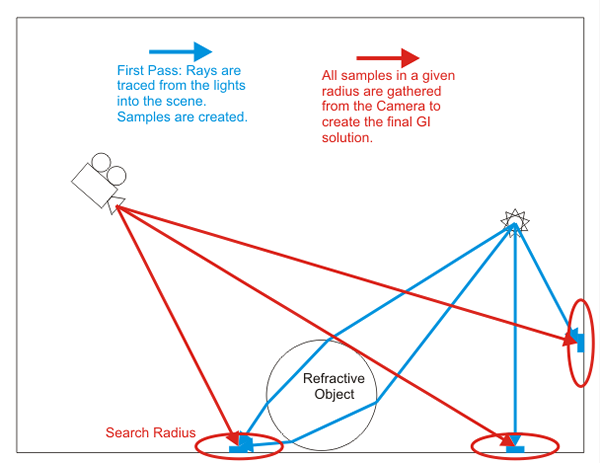
\includegraphics[width=0.75\linewidth]{img/pmDiagram.png}
\caption{\label{img:pmdiag} Photon Mapping Algorithm}
\end{figure}

This algorithm, unlike all the previously mentioned algorithms, introduces bias, because there is an approximation of the photon map search area to an infinity small area. This causes the algorithm to not converge to the correct result but to an approximation with an unknown error (bias).

Although biased, this algorithm performs well in the handling of caustics, even reflected and refracted caustics. However, the convergence rate for the overall diffuse illumination is smaller than that of Bidirectional Path Tracing \citep{Georgiev}. Another back draw of this algorithm is memory usage, since the more photons used to rendering, the larger the photon map has to be.

\subsection{Progressive Photon Mapping}

Photon Mapping is a biased algorithm, although if the number of photons used tends to infinity and the search radius in the photon map tends to zero, the bias is zero in the limit. This makes the bias in the algorithm consistent and this property can be used to improve the quality of the algorithm.

Instead of storing the positions of photons in the photon map, the hit points from the camera rays are stored in an acceleration structure. Then, when photons are traced from the light sources, a range search looks for any hit point in the neighborhood and the contribution of that photon is added to the corresponding pixels. In each iteration of the algorithm the search radius is decreased according to a constant parameter of the algorithm \citep{Hachisuka}.

\begin{figure}[H]
\centering
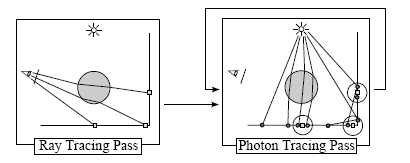
\includegraphics[width=0.75\linewidth]{img/ppmDiagram.png}
\caption{\label{img:ppmdiag} Progressive Photon Mapping Algorithm}
\end{figure}

This alteration to the algorithm improves the efficiency of Photon Mapping, namely in terms of memory usage, now fixed proportional to the size of the image, instead of proportional to the number of photons used. Although with \gls{ppm} the bias may be zero in the limit, this algorithm also produces more useless work the longer it runs, since as the search radius decreases with the execution, more photons are traced that do not contribute to the final image.

\subsection{Bidirectional Photon Mapping}

In order to increase the robustness of the Photon Mapping technique, \cite{Vorba} proposed the \gls{bpm} algorithm. Instead of using a heuristic to determine the use of final gather and direct photon map consult, this algorithm uses \gls{mis} in order to increase the robustness of the algorithm, mostly when glossy materials are present.

This algorithm operates mostly like \gls{pm} but using only one photon map. In the rendering phase, instead of tracing only primary rays, a whole path is traced, and at every intersection of this path the photon map is consulted. During this step every photon contribution is independently weighted according to the probability it was generated.

This algorithm can also be progressive by reducing the search radius of the photon map at each iteration.

\section{Vertex Connection and Merging}

This new algorithm proposed by \cite{Georgiev}, combines two complementary algorithms in order to create a more robust rendering algorithm. As seen previously, Bidirectional Path Tracing has high convergence rate and can handle most types of illumination effects, however it has problem rendering reflected or refracted caustics. On the other hand, the family of Photon Mapping algorithms has no problem dealing with caustics but has an overall low convergence rate. The combination of these two algorithms into a new one, Vertex Connection and Merging, through \gls{mis} is much more robust than the original algorithms alone.

The combination of Photon Mapping and Bidirectional Path Tracing required the reformulation of one of these algorithms, since they calculate the image values through different mathematical frameworks: while Bidirectional Path Tracing calculates an integral on the path space, Photon Mapping calculates a photon density estimation. To achieve this, Photon Mapping was reformulated as a path sampling technique, where a path is successfully sampled if the last vertex of the light sub-path falls into the search area of a vertex from the camera sub-path. These two vertices are effectively merged so the last vertex in the light sub-path is not considered part of the generated path itself but only as a conditional test of the acceptance of this new path. For this new path sampling technique, called Vertex Merging, an associated probability density function is needed to use multiple importance sampling. 
\begin{equation}
p_{VM}=[\pi r^2 p(x_{s-1}\xrightarrow{}x_{s}^{*})]p_{VC}(x)
\label{eq:pvm}
\end{equation}
where $p_{VC}(x)$ is the probability of generating path $x$ through Bidirectional Path Tracing and the initial part is the probability density function for the last light sub-path vertex to intersect the merging area of the last camera sub-path vertex.

\begin{figure}[H]
\centering
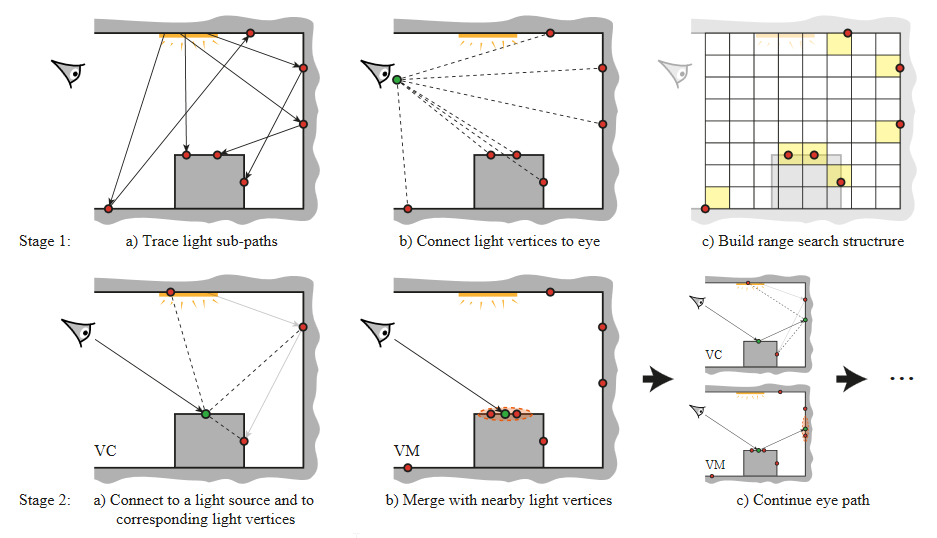
\includegraphics[width=\linewidth]{img/vcmDiagram.png}
\caption{\label{img:vcmdiag} Vertex Connection and Merging Algorithm}
\end{figure}

With a new path sampling technique, Vertex Merging, in conjunction with Bidirectional Path Tracing, or Vertex Connection, it is possible to combine these two techniques using \gls{mis} to achieve robustness. This new combined algorithm starts like Bidirectional Path Tracing by tracing a set of paths from the light sources, and stores the vertices in a range search acceleration structure. Then when the camera sub-paths are being traced, each vertex of the camera sub-path is connected to all the vertices of the respective light sub-path, and searches the acceleration structure for any vertices from any light sub-path viable for merging.

This combined light transport algorithm maintains the high convergence rate of Bidirectional Path Tracing, while being able to handle caustics efficiently like Photon Mapping. The efficiency of this algorithm can still be improved by applying \gls{mcmc} techniques on top of it \citep{Georgiev}.

\section{Heterogeneous Systems}

An heterogeneous system is a computing system with different processing devices with different architectures. Indeed, most average computers are heterogeneous systems that contain a multicore \gls{cpu} used for most tasks and a massively parallel \gls{gpu} used mainly for graphics rasterization.  In order to achieve peak performance on each type of device, there are specific architecture dependent optimizations that must be implemented by programmers.

When programming \gls{cpu}'s, most parallelism is implicit, in the form of instruction parallelism and the use of vectorial instructions(\gls{simd}). The use of vectorial instructions is critical in order to achieve peak performance, and although the compiler may perform the automatic vectorization of the code, the code must follow a strict pattern for this to happen. \gls{cpu} performance is also dependent on its memory hierarchy model with few registers and a large main memory, with some levels of cache memory to amortize the time cost of accessing the main memory. It is though imperative to use memory locality to avoid cache misses and accessing the main memory which is much slower than accessing the cache memory. Further issues arise with memory hierarchy when introducing thread level parallelism. When multiple cores have a cache line stored in their private cache and that line is altered by one of them, that cache line has to be invalidated and reloaded on all other caches in order to avoid a incoherent state.

Programming \gls{gpu}

These two processors have separate addressing spaces, communication between them is costly, and even the programming model is different between them. This imposes difficulties to developers and inhibits portability of the code across different platforms \citep{Kunzman}. However there are potential performance gains in using both devices since there is additional computational power available. 



\subsection{DICE}

Developing applications for heterogeneous platforms is a difficult task as explained previously. DICE \citep{Barbosa} is an application framework for developing heterogeneous applications that aims to ease the process of development for heterogeneous platforms containing both \gls{cpu} and \gls{gpu}, with an emphasis on irregular workloads.

%DICE uses a task model in which tasks are scheduled by the system throughout the various available processors. The workload is distributed by generating sub-tasks of finer granularity and assigning them to different processors. The main features of DICE are an adaptative scheduler that analyses the execution time of each submited task and uses that information to perform load balancing operations, and a memory manager that simplifies different addressing spaces by presenting the developer only one address space and transparently preforming copies between different addressing spaces whenever required \citep{Barbosa}.

DICE uses a task driven model that schedules work across processing devices through a granularity refinement. When a task is submitted to the scheduler, sub-tasks of finer granularity are generated and executed on the available devices. This scheduler analyses the execution time of the task on each device to enhance the workload distribution in order to attain maximum performance. DICE also provides a virtual shared memory manager that abstracts different addressing spaces by presenting the developer only one address space and transparently performing copies between different addressing spaces whenever required.

DICE tasks support a variety of execution modes. The developer can provide a single kernel and the task can execute automatically on \gls{cpu} and \gls{gpu}, while it is also possible to provide the task with specialized code for each architecture. The specialized \gls{gpu} implementation can be provided as a CUDA kernel or as a call to specialized libraries. These possibilities allow a simple programming model while retaining the possibility of refinement, architecture specific optimizations and the use of external optimized libraries.

\subsection{StarPU}

%\todo[inline]{talk about starPU concurrent work}

%StarPU is a framework that provides high-level programming abstractions, integrated data management and enhanced scheduling mechanisms. It also provides an unified execution model working together with dynamic scheduling policies. The run-time features a data management system that entails several features: automatic work decomposition and data transfers, communication and computation overlapping, data pre-getching and locality aware scheduling, among others. StarPU has davanced data management and sophisticated scheduling techniques, such as the Heterogeneous Earliest Finish Time approach.

StarPU \citep{augonnet2011starpu} is a framework whose goal is similar to DICE. It amis to provide high level abstractions of an heterogeneous system, providing data management facilities and enhanced scheduling mechanisms, such as the Heterogeneous Earliest Finish Time approach. The data management system provides features such as automatic work decomposition, transparent data transfers between devices, communication and computation overlapping data pre-fetching and locality aware scheduling, among others.
\chapter{The Problem and its Challenges}

In this project, the main goals are to evaluate the relative performance and robustness of different light transport algorithms, as well as to evaluate their suitability to heterogeneous systems and evaluate the DICE framework in terms of performance and usability. To this effect, different implementations of the previously mentioned light transport algorithms will be developed for both \gls{cpu} and \gls{gpu} using specialized ray tracing frameworks targeted to the different devices: Optix targeted for \gls{gpu} and Embree for \gls{cpu}. The performance of the algorithms will be evaluated by comparing the image quality for a given rendering time and by measuring the rendering time needed to achieve a given image quality. In addition to this, the overhead of using the DICE framework will be measured and compared to the gain of using various devices. In a first stage of developent, all the algorithms will be developed independently for \gls{cpu} and \gls{gpu}. Then in a second stage, these implementations will be integrated in DICE for use in heterogenous systems. Finally all the performance measurements will be compared in order to evaluate all the previous points.

As mentioned before, communication between different devices hinders performance, and although most algorithms require no synchronization, photon mapping requires sharing the photon map across all devices, or else there would be different variance through the image, which is a perceptible flaw. As \gls{vcm} generates a new photon map in each iteration, this photon map must be copied to all used devices in every iteration, which may negatively affect performance. Another challenge is the usage of different data structures by the different ray tracing frameworks which adds complexity to the development process.


\chapter{Experimental Results}

\section{Technical Aproach}

In order to evaluate the suitability of advanced light transport algorithms to heterogeneous systems, optimized implementations of all algorithms were developed for both \gls{cpu} and \gls{gpu}. These implementations were developed using specialized ray tracing libraries, namely Nvidia Optix \citep{parker2010optix} and Intel Embree \citep{wald2014embree}.


There are two possible shcemes of work decomposition across devices. One is image space decomposition, where each device processes a portion of the image pixels. Another possible alternative is to distribute the algorithm iterations across the devices. In \gls{pt} and \gls{bdpt} the choice between these two approaches is almost irrelevant, however in photon based algorithms (\gls{bpm} and \gls{vcm}) it is not that simple. If image plane division was applied, it would force communication between the \gls{cpu} and the \gls{gpu} in every iteration. If an iteration division was applied, for every \gls{cpu} core a complete photon map would be stored in the main memory.

In order to solve these issues, DICE was configured to consider all the \gls{cpu} cores as a monolithic device, leaving the distribution of work in the \gls{cpu} to the application code. The work between the \gls{cpu} and the \gls{gpu} is then distributed in a set of independent iterations, eliminationg all communication needs. Between the \gls{cpu} cores the image plane is divided, eliminating the excesive memory use. This approach was applied to every developed algorithm in order to ease development and to allow an algorithm independent DICE configuration.

%Integrating both \gls{cpu} and \gls{gpu} implementations using DICE was simple, although some adaptations were applied in order to improve efficiency. DICE considers every \gls{cpu} core as an independant device, the same way it considers a \gls{gpu} for the purpose of work sharing. However, for photon mapping based algorithms this is innapropriate because if image plane division was applied, it would force communication between the \gls{cpu} and the \gls{gpu} in every iteration. If an iteration division was applied, for every \gls{cpu} core a complete photon map would be stored in the main memory. In order to solve these issues, DICE was configured to consider all the \gls{cpu} cores as a monolithic device, leaving the distribution of work in the \gls{cpu} to the application code. The work between the \gls{cpu} and the \gls{gpu} is then distributed in a set of independent iterations, eliminationg all communication needs. Between the \gls{cpu} cores the image plane is divided, eliminating the excesive memory use.



\section{Methodology}

In order to test the scalability and efficiency of the studied algorithms, the execution times of the studied algorithms were measured using only the \gls{gpu}, and while using only the \gls{cpu} or both, with a varying number of \gls{cpu} cores and threads per core, in order to evaluate the gain of using \gls{ht}. Every time measurement was executed five times, selecting the best time as the final result. The workload distribution between the devices was also measured by the DICE scheduler at the end of the five time measurements, being the final result the best possible distribution calculated by DICE. These results represent the fraction of iterations assigned to each device, which may not be a good performance evaluation metric since the iteration time is not uniform, specially in photon mapping based algorithms, in which the iteration time is dependent on the search radius, which decreases in every iteration. These tests were executed using the Living Room Scene with a resolution of 1024x768 and 50 samples per pixel.

In order to evaluate the image quality produced by the studied algorithms, three scenes were used for testing, each with a different goal. The Sponza scene, courtesy of Crytek, is an outdoor scene with only diffuse materials, but complex geometry nonetheless. The Kitchen scene from Lux Renderer, is an indoor scene with glossy materials. The final and most complex scene, the Living Room, courtesy of Iliyan Georgiev, is an indoor scene as well but with an emphasis on reflected caustics and complex lighting. For every scene a reference image was rendered with \gls{vcm} with 100000 samples per pixel. Then for every algorithm a set of images with an approximate rendering time were produced. All these images were compared to the reference image using the \gls{rmse} metric.

\begin{figure}[h]
\centering
\begin{minipage}[b]{0.3\linewidth}
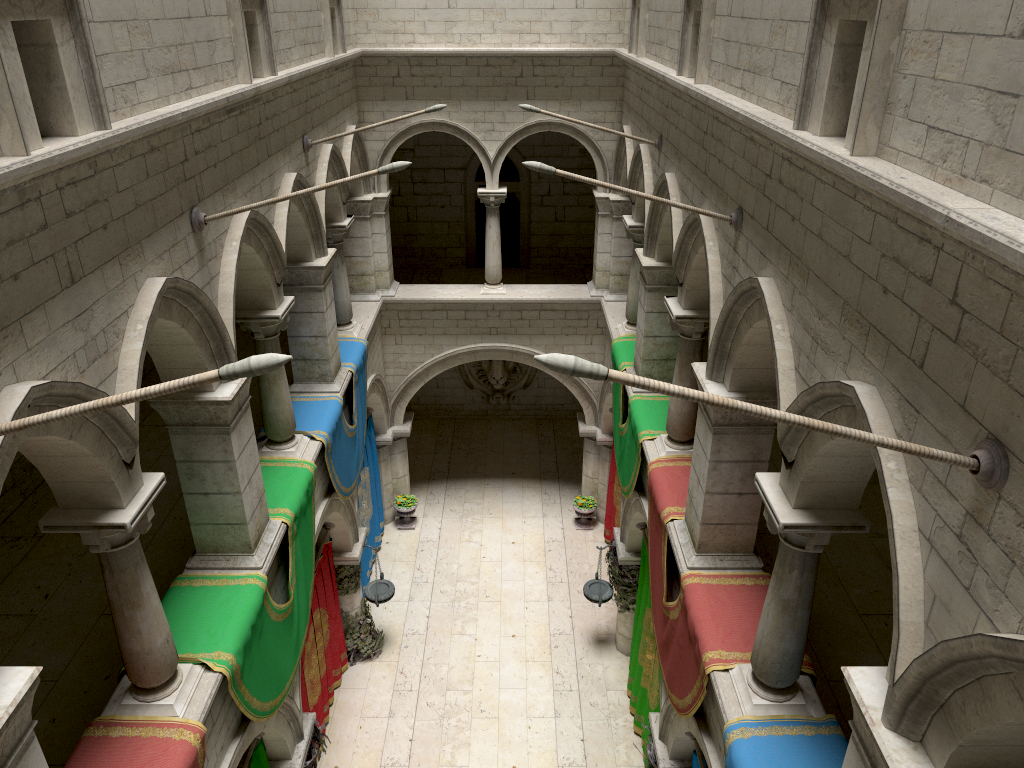
\includegraphics[width=\linewidth]{img/sponza_ref.jpg}
\caption{\label{img:sponza_ref} Sponza scene reference image.}
\end{minipage}
\quad
\begin{minipage}[b]{0.3\linewidth}
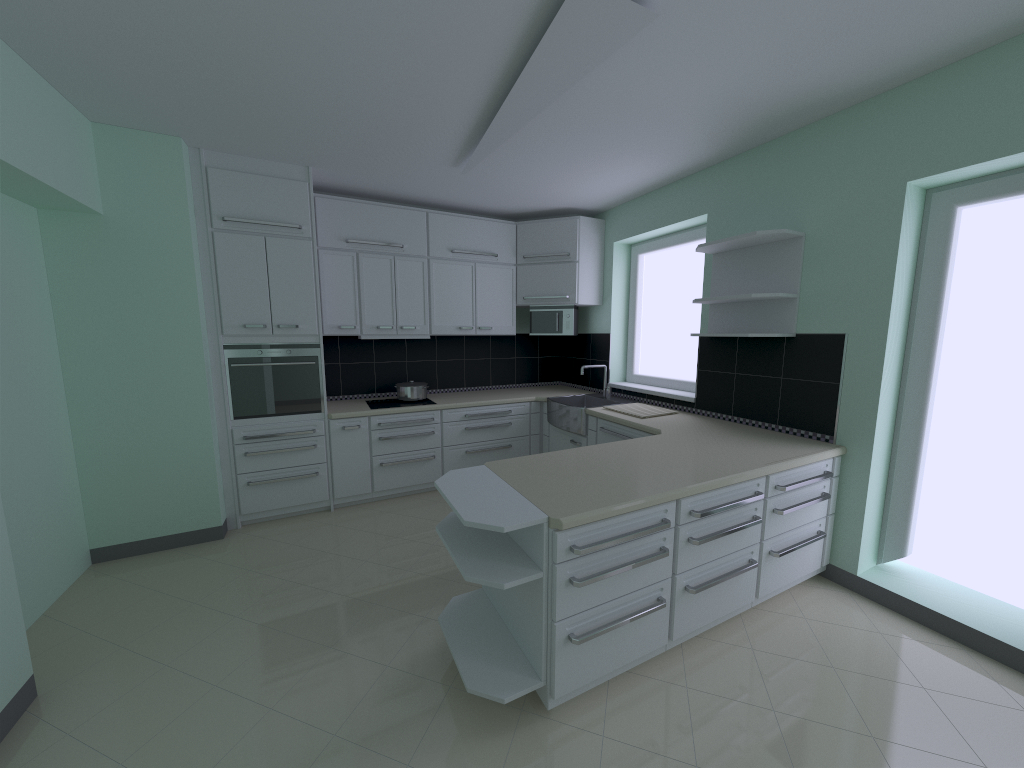
\includegraphics[width=\linewidth]{img/kitchen_ref.jpg}
\caption{\label{img:kitchen_ref} Kitchen scene reference image.}
\end{minipage}
\quad
\begin{minipage}[b]{0.3\linewidth}
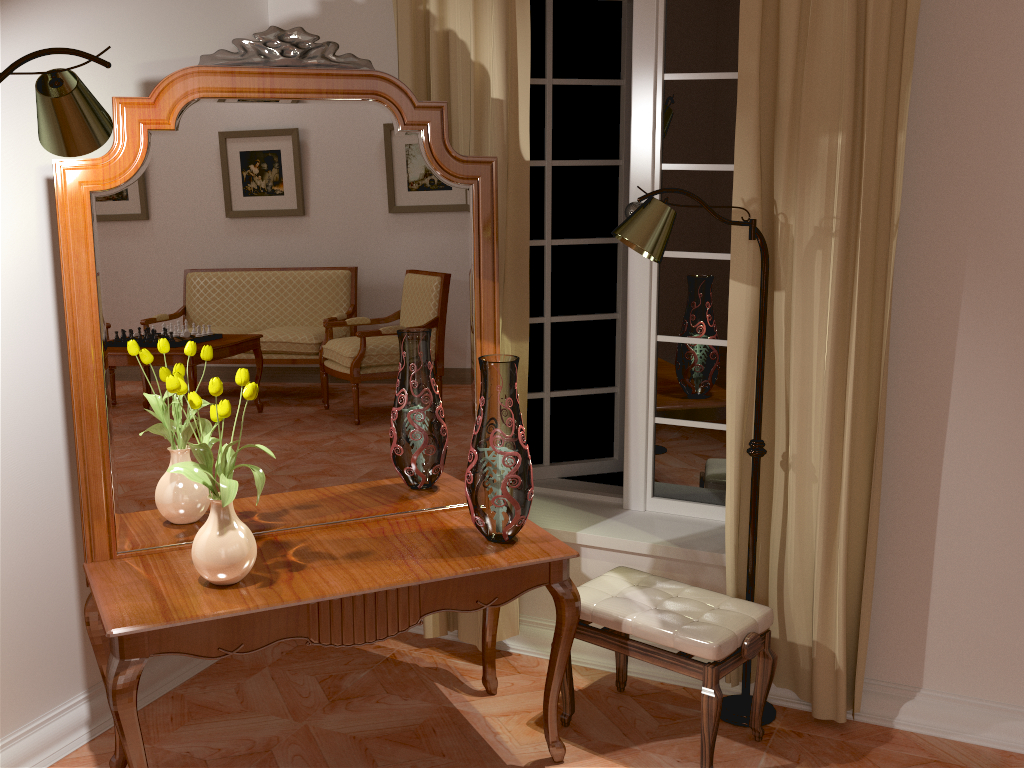
\includegraphics[width=\linewidth]{img/livingroom_ref.jpg}
\caption{\label{img:livingroom_ref} Living Room scene reference image.}
\end{minipage}

\end{figure}

\section{Experimental Setup}

All experiments were executed on a dual-socket computer with two 10 core Intel Xeon E5-2670 v2 \gls{cpu} at the frequency of 2.50GHz, 64 GB of RAM and a Nvidia Tesla K20 \gls{gpu}.

Every software used was updated to the versions listed in table~\ref{tab:soft_ver}.

\begin{table}[h]
\centering
\begin{tabular}{|l|l|}

\hline
Software & Version \\
\hline
Linux & 2.6.32-279 \\
\hline
GCC & 4.8.2 \\
\hline
CUDA Toolkit & 5.5 \\
\hline
Optix & 3.7 \\
\hline
Embree & 2.5.1 \\
\hline

\end{tabular}
\caption{\label{tab:soft_ver} Software Used}
\end{table}

\section{Result Analisys}

\subsection{\label{sec:texec}Excution Time Results}

\begin{figure}[H]
\centering
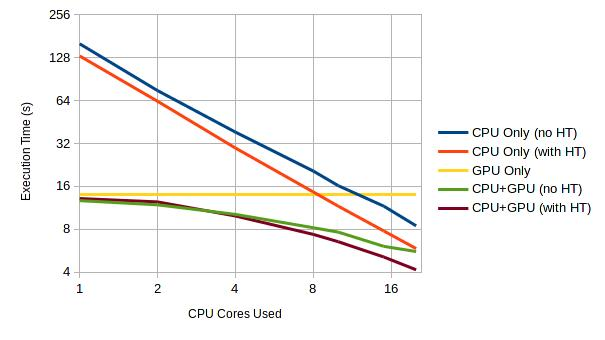
\includegraphics[width=0.8\linewidth]{img/ptTexec.jpg}
\caption{\label{img:ptTexec} Path Tracer Execution Times}
\end{figure}

\begin{figure}[H]
\centering
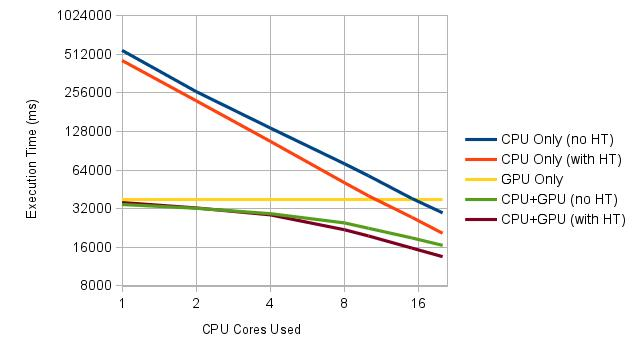
\includegraphics[width=0.8\linewidth]{img/bptTexec.jpg}
\caption{\label{img:bptTexec} Bidirectional Path Tracer Execution Times}
\end{figure}

\begin{figure}[H]
\centering
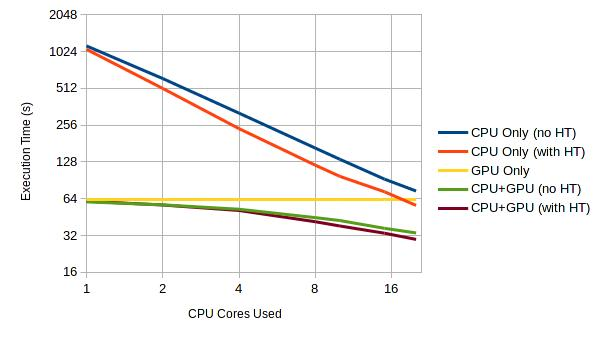
\includegraphics[width=0.8\linewidth]{img/bpmTexec.jpg}
\caption{\label{img:bpmTexec} Bidirectional Photon Mapping Execution Times}
\end{figure}

\begin{figure}[H]
\centering
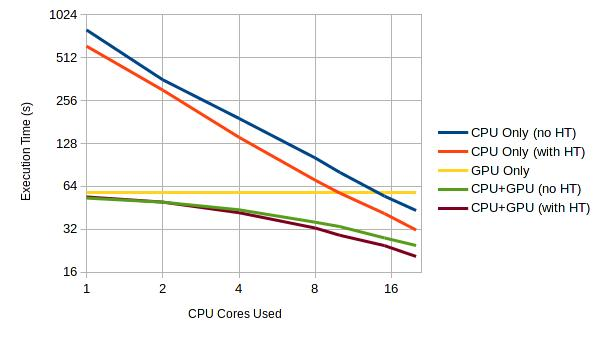
\includegraphics[width=0.8\linewidth]{img/vcmTexec.jpg}
\caption{\label{img:vcmTexec} VCM Execution Times}
\end{figure}

All the execution times measured indicate that all the algorithms studied are scalable and take advantage of both devices in the rendering process. Note that no inflection point was reached, i.e., a point above which execution time starts increasing with additional processing devices. Unfortunately, we were unable to further increase the number of devices in order to detect such inflection point.

\subsection{CPU Speedup Results}

Due to the lack of a clear speedup definition for heterogeneous systems, here is presented only the speedup for the \gls{cpu} implementation. However, in section ~\ref{sec:hefficiency} there is presented an heterogeneous analisys.

\begin{figure}[H]
\centering
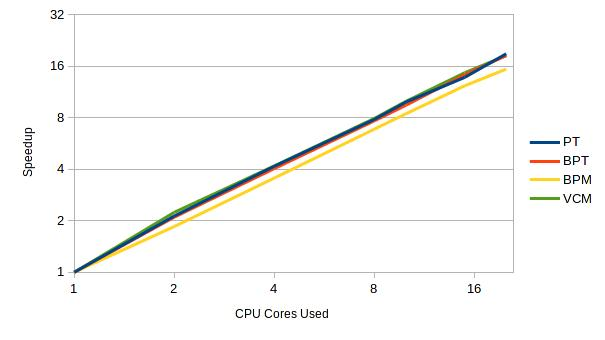
\includegraphics[width=0.8\linewidth]{img/speedup.jpg}
\caption{\label{img:speedup} Speedup Analisys}
\end{figure}

Every algorithm except Bidirectional Photon Mapping achieve an almost linear speedup, while this only achives a speedup of 15.4 using 20 cores. Although not present in this plot, all algorithms seem to take advantage of Hyper Threading, which increases the overall performance between 30\% to 50\%.

\subsection{CPU Parallelization Eficiency Results}

Due to the lack of a clear efficiency definition for heterogeneous systems, here is presented only the efficiency for the \gls{cpu} implementation. However, in section ~\ref{sec:hefficiency} there is presented an heterogeneous analisys.

\begin{figure}[H]
\centering
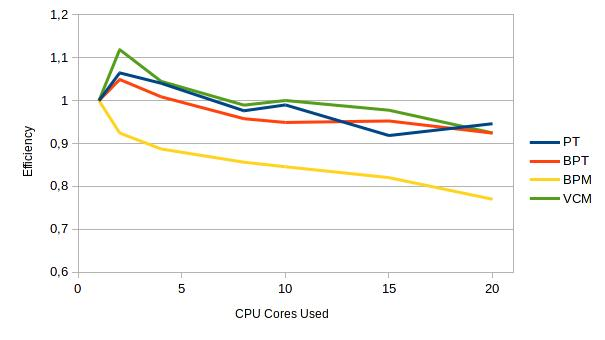
\includegraphics[width=0.8\linewidth]{img/efficiency.jpg}
\caption{\label{img:efficiency} Efficiency Analisys}
\end{figure}

Every algorithms except Bidirectional Photon Mapping has a parallelization efficiency above 0.9, while this falls to an efficiency of 0.77 using 20 cores. This inefficiency may be due to the high memory access this algorithm has compared to all the other algorithms. Note that even though efficiency drops with increased resources, as expected, the inflection point referred in section ~\ref{sec:texec} is still far from being reached.

\subsection{Workload Distribution Results}

\begin{figure}[H]
\centering
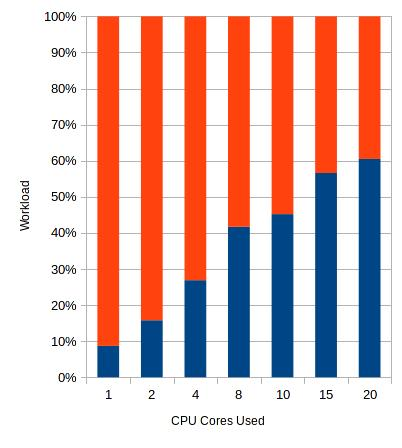
\includegraphics[width=0.8\linewidth]{img/ptwl.jpg}
\caption{\label{img:ptwl} Path Tracer Workload Distribution}
\end{figure}

\begin{figure}[H]
\centering
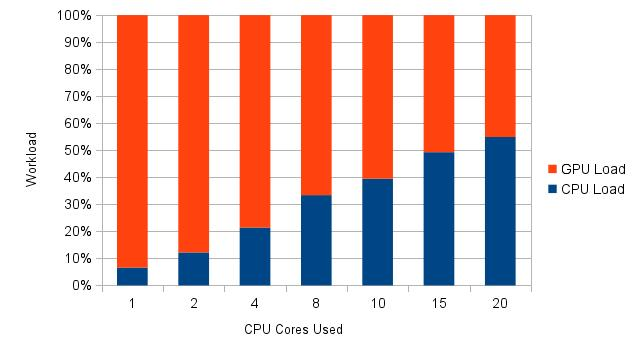
\includegraphics[width=0.8\linewidth]{img/bptwl.jpg}
\caption{\label{img:bptwl} Bidirectional Path Tracer Workload Distribution}
\end{figure}

\begin{figure}[H]
\centering
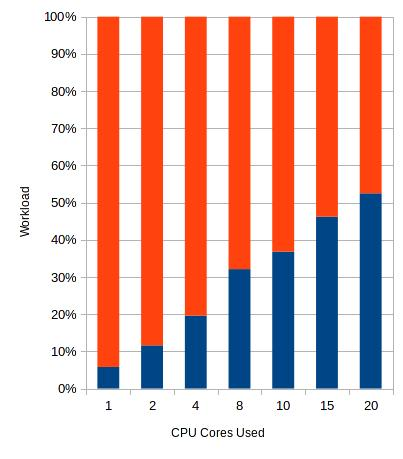
\includegraphics[width=0.8\linewidth]{img/bpmwl.jpg}
\caption{\label{img:bpmwl} Bidirectional Photon Mapping Workload Distribution}
\end{figure}

\begin{figure}[H]
\centering
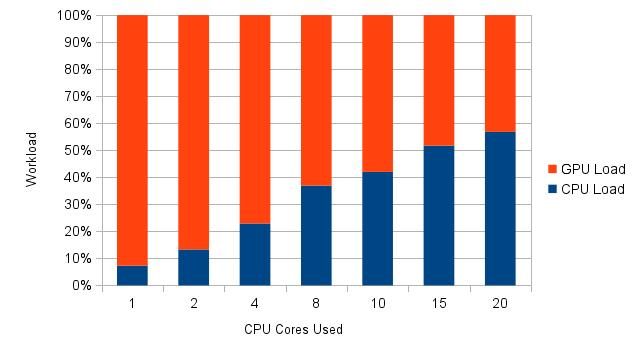
\includegraphics[width=0.8\linewidth]{img/vcmwl.jpg}
\caption{\label{img:vcmwl} VCM Workload Distribution}
\end{figure}

As had been shown by all previous performance metrics these four figures clearly show that the algorithms are able to scale as the number of CPU cores increases. The relative workload processed by the CPU increases with the number of cores, demonstrating that all devices are being used. This behaviour is true and similar for all the four algorithms.

\subsection{\label{sec:hefficiency} Heterogeneous Efficiency}

Although all previous metrics seem to indicate that the tested algorithms use all the resources efficiently, there was no absolute measurement of how well the resources were used.

\cite{Chamberlain98} defined heterogeneous speedup according to equation ~\ref{eq:HetSpeedUp}, where $T_{\mbox{\tiny ref}}$ is a reference execution time and $T_D$ is the execution time on an hetereogeneous system constituted by the set $D$ of devices.

\begin{equation}
S_h(D) = \frac{T_{\mbox{\tiny ref}}}{T_D}
\label{eq:HetSpeedUp}
\end{equation}

The optimal heterogeneous speedup, $S_h^*(D)$, can not be defined as function of the number of used devices, because different devices offer different amounts of computational power. \cite{Chamberlain98} expressed this ideal speedup as a ratio of computing rates. 

Being the computing rate for the device $d \in D$ for a given workload $W$ be $R_d = \frac{W}{T_d}$, then the ideal computing rate is the sum of all the computing rates of all the devices $d \in D$.

\begin{equation}
R^*_D = \sum_{d \in D} R_d = W \sum_{d \in D} \frac{1}{T_d}
\label{eq:StarCapacity}
\end{equation}

\cite{Chamberlain98} define $S_h^*(D)$ as the ratio between available computing rate and the computing rate of the reference device:

\begin{equation}
S^*_h(D) = \frac{R^*_D}{R_{\mbox{\tiny ref}}} = T_{\mbox{\tiny ref}} \sum_{d \in D} \frac{1}{T_d}
\label{eq:StarHetSpeedUp}
\end{equation}

Given the definitions of heterogeneous speedup and optimal heterogeneous speedup (equations \ref{eq:HetSpeedUp} and \ref{eq:StarHetSpeedUp}), heterogeneous efficiency can thus be defined as the ratio of both

\begin{equation}
E_h(D) = \frac{S_h(D)}{S_h^*(D)} = \frac{R_D}{R^*_D} = \frac{\frac{1}{T_D}}{\sum_{d \in D} \frac{1}{T_d}}
\label{eq:HetEff}
\end{equation}

Given these definitions, it is possible to calculate the efficiency of the heterogeneous implementations using one \gls{gpu} and a varying number of \gls{cpu} cores, as depicted in the figure ~\ref{img:hefficiency}.

\begin{figure}[H]
\centering
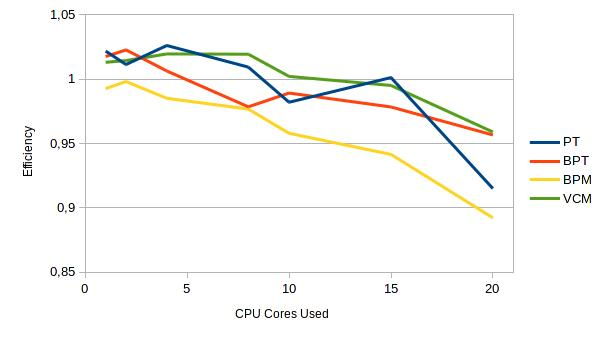
\includegraphics[width=0.8\linewidth]{img/hefficiency.jpg}
\caption{\label{img:hefficiency} Heterogeneous Efficiency Analisys}
\end{figure}

All algorithms achive an heterogeneous efficiency above 0.9, except \gls{bpm}. As with \gls{cpu} efficiency, even though it drops with the increase of resourses, an inflection point is far from being reached.

\subsection{Image Quality Results}

\begin{figure}[H]
\centering
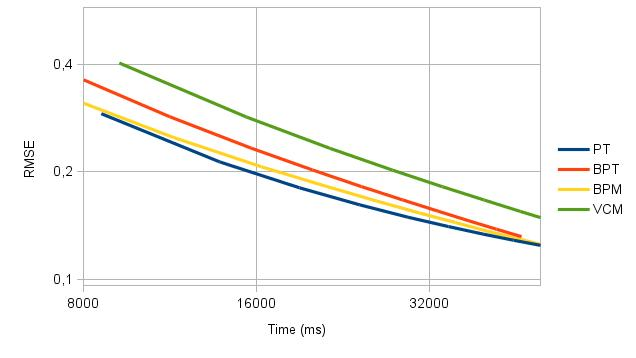
\includegraphics[width=0.8\linewidth]{img/sponzaImgq.jpg}
\caption{\label{img:sponzaImgq} Sponza Image Quality}
\end{figure}

\begin{figure}[H]
\centering
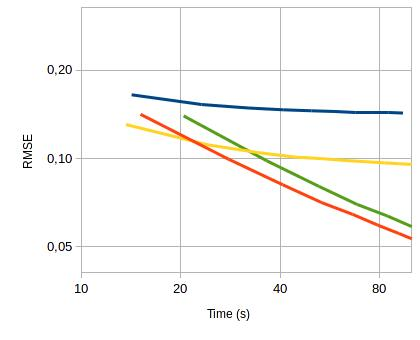
\includegraphics[width=0.8\linewidth]{img/kitchenImgq.jpg}
\caption{\label{img:kitchenImgq} Kitchen Image Quality}
\end{figure}

\begin{figure}[H]
\centering
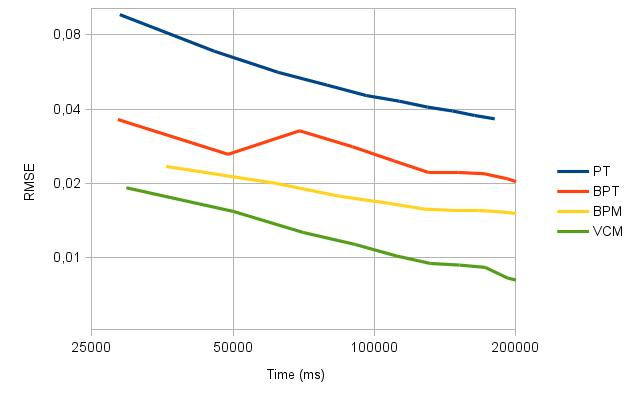
\includegraphics[width=0.8\linewidth]{img/livingroomImgq.jpg}
\caption{\label{img:livingroomImgq} Livingroom Image Quality}
\end{figure}

In the Sponza scene, all algorithms seem to converge to the right solution, however Path Tracing is the best algorithms in this case. This may be due to the outdoor scene configuration where many of the light paths traced are lost and miss the scene, as well as the simple material lighting which is completely captured by Path Tracing, not needing more complex solutions.

In the Kithcen scene, both Bidirectional Path Tracer and Vertex Connecion and Merging algorithms converge to the expected result, although the former is faster for this scene. Both Path tracer and Bidirectional Photon Mapping present lower convergence rates due to the high variance of the lighting effects present, namely caustics incident on glossy surfaces.

In the Living Room scene, Vertex Connection and Merging has the fastest convergence, while the remaining algorithms converges much more slowly. This happened due to the presence of many specular-diffuse-specular paths (namely the reflected caustics in the mirror), which \gls{vcm} was specially designed to capture.

%\part{Core of the dissertation}


		
\bookmarksetup{startatroot} % Ends last part.
\addtocontents{toc}{\bigskip} % Making the table of contents look good.
\cleardoublepage

%----------------- Bibliography (needs bibtex) --------------------------------%
\bibliography{dissertation}
%----------------- Index of terms (needs  makeindex) --------------------------%
\printindex
%------------------------------------------------------------------------------%
	
	\appendix
	\renewcommand\chaptername{Appendix}

	% Add appendix chapters

%\part{Apendices}


	
\end{document}

